\documentclass{article}

% if you need to pass options to natbib, use, e.g.:
% \PassOptionsToPackage{numbers, compress}{natbib}
% before loading nips_2016
%
% to avoid loading the natbib package, add option nonatbib:
% \usepackage[nonatbib]{nips_2016}

\usepackage[final]{nips_2016}

% to compile a camera-ready version, add the [final] option, e.g.:
% \usepackage[final]{nips_2016}

\usepackage[utf8]{inputenc} % allow utf-8 input
\usepackage[T1]{fontenc}    % use 8-bit T1 fonts
\usepackage{hyperref}       % hyperlinks
\usepackage{url}            % simple URL typesetting
\usepackage{booktabs}       % professional-quality tables
\usepackage{amsfonts}       % blackboard math symbols
\usepackage{nicefrac}       % compact symbols for 1/2, etc.
\usepackage{microtype}      % microtypography

\usepackage{graphicx}
\usepackage{subcaption}
\usepackage{enumitem}
\usepackage{url}
\usepackage{amsmath}

% CleverRef Setup
\usepackage[capitalize,noabbrev]{cleveref}

\title{Parallel Sparse Convolution for Deep Learning}

% The \author macro works with any number of authors. There are two
% commands used to separate the names and addresses of multiple
% authors: \And and \AND.
%
% Using \And between authors leaves it to LaTeX to determine where to
% break the lines. Using \AND forces a line break at that point. So,
% if LaTeX puts 3 of 4 authors names on the first line, and the last
% on the second line, try using \AND instead of \And before the third
% author name.

\author{
  Ravi Teja Mullapudi 
  \And
  Prashanth Menon
}

\begin{document}
% \nipsfinalcopy is no longer used

\maketitle

\begin{abstract}
Performing inference on high-resolution video and image data using
state-of-the-art deep vision models is computationally demanding.  At the
heart of deep learning models for computer vision is the convolution
operation which is a 3D filtering operation on high-dimensional features.
Improving the performance of convolution layers continues to be a key aspect
of enabling computer vision research. There have been several efforts to
improve the efficiency by switching to different representation domain (FFT,
Winograd).  Though transformations into different domains enables performing
fewer expensive operations, they do not account for the possibility of only
needing to perform the convolution sparsely across the image (the domain
transformation significantly reduces the sparsity). Given the high
redundancy between video frames or the sparse signal generated by sensors
like LIDAR one can determine the sparse spatial locations to perform the
convolution. In this project, we demonstrate that a simple parallel and
locality-aware implementation of sparse convolution is indeed competitive
with highly-tuned vendor implementations of dense convolutions which operate
in a transformed domain.
\end{abstract}

\newcommand{\floor}[1]{\lfloor #1 \rfloor}

\section{Background and Related Work}
\label{sec:bg-rw}
\textbf{Convolution Layer} 
The filtering operation typically used in convolutional neural networks referred
to as the convolution layer is shown in Equation~\ref{eqn:conv}. The operation
takes as input features $I$, the filter coefficients $F$, and produces the
output features $O$.

\begin{equation}
O_{b, h, w, k} = \sum_{z=0}^{C}\sum_{x=0}^{F_h} \sum_{y=0}^{F_w} I_{b, S h+x, S w+x, z} * F_{k, z, x, y}
\label{eqn:conv}
\end{equation}

The features and the filter coefficients are represented as 4d tensors of the
following shapes:
\begin{align*}
& I:B \times H \times W \times C \\
& O:B \times (\floor{(H - F_h + 2P)/S} + 1) \times (\floor{(W - F_w + 2P)/S} +
    1) \times K \\
& F:C \times K \times F_h \times F_w
\end{align*}
$B$ is the size of the batch of input features. $H$ and $W$ are the spatial
height and width of the input feature map. $S$ is the spatial stride at which
the filtering is performed on the input (sampling rate). $P$ is the amount of
padding added to the input to handle boundary conditions. $F_h$ and $F_w$ are
the spatial height and width of the filters. $C$ and $K$ are the input and output
feature dimensions respectively. 

\textbf{Spatial Sparsity} In settings where the input data is sparse or highly
redundant (consecutive frames of video) the convolution operation can only
performed in spatial locations where the input signal is present or changes
significantly. Figure~\ref{fig:frames} shows frames captured from one of the
onboard cameras in an autonomous driving car moving. Despite being captured a
low frame rate there is a significant region of the input that remains unchanged
at the pixel level. Feature representations in deeper layers of a network are
more robust to pixel-level changes and would exhibit even higher levels of
sparsity~\cite{shelhamer2016clockwork}.

\begin{figure}[h]
	\centering
\begin{subfigure}{0.3\textwidth}
	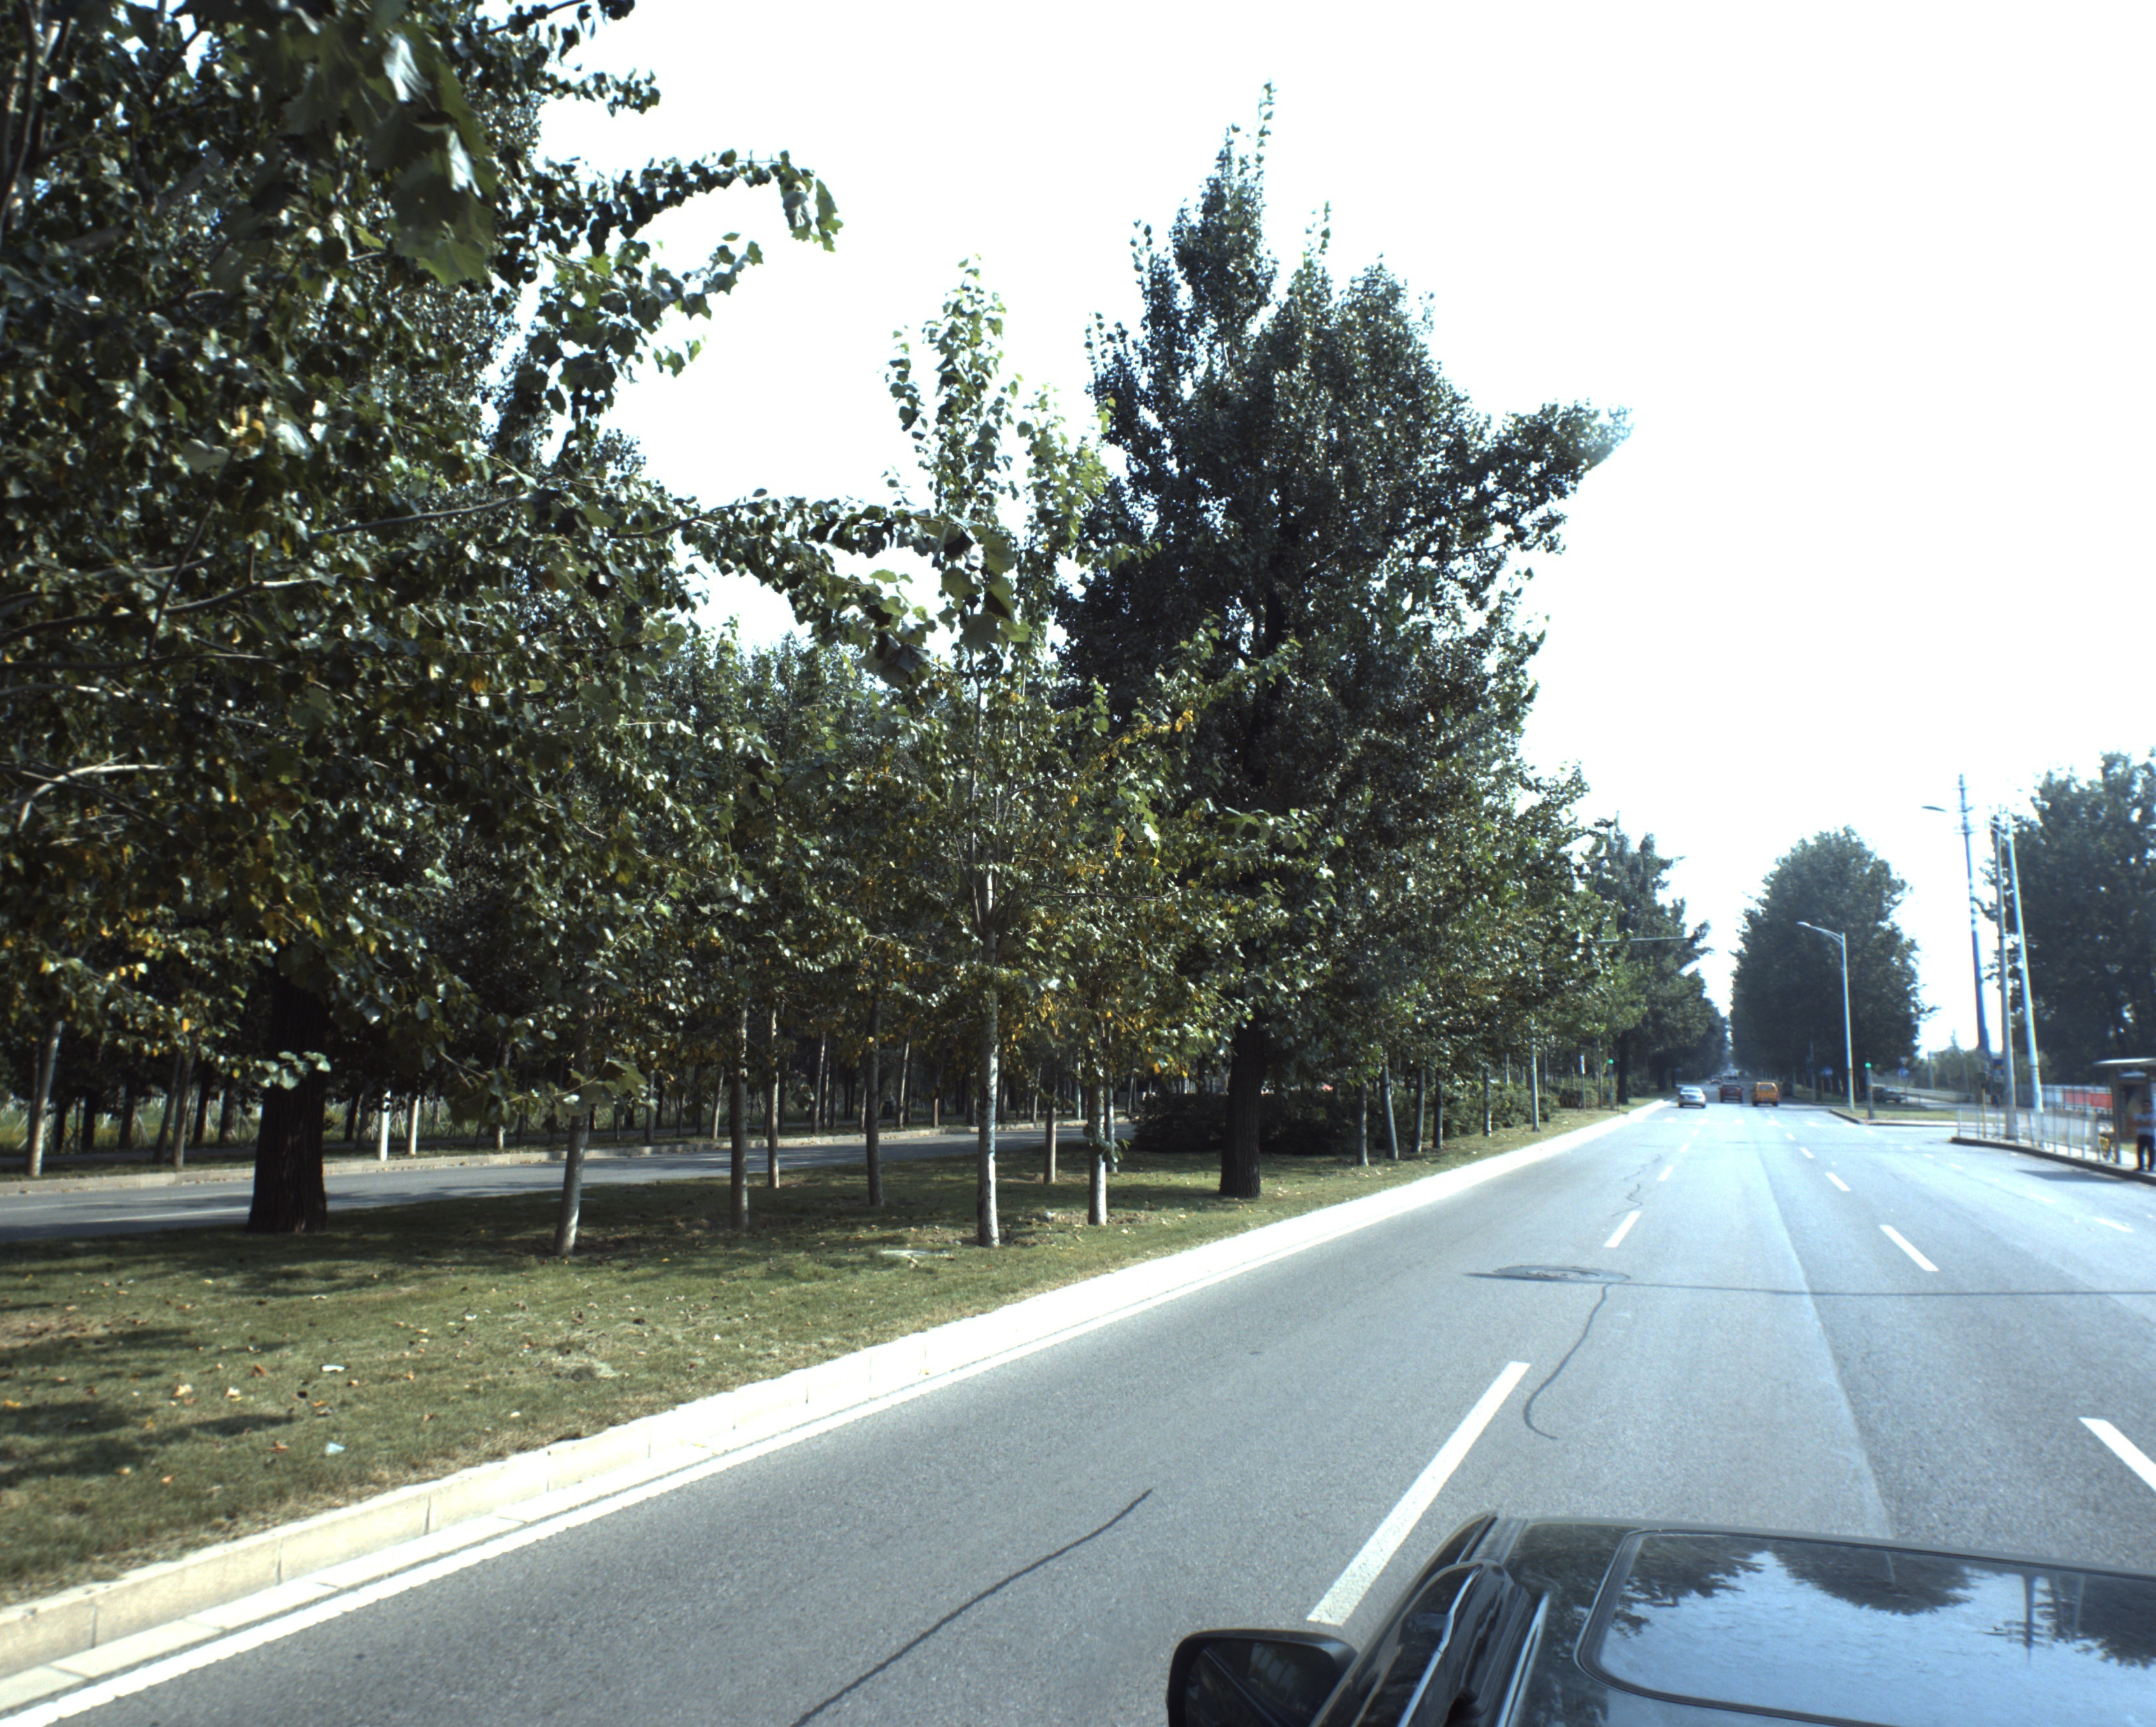
\includegraphics[width=\textwidth]{170908_061541883_Camera_5.jpg}
	\caption{Frame $n$}
\end{subfigure}
\hspace{0.1in}
\begin{subfigure}{0.3\textwidth}
	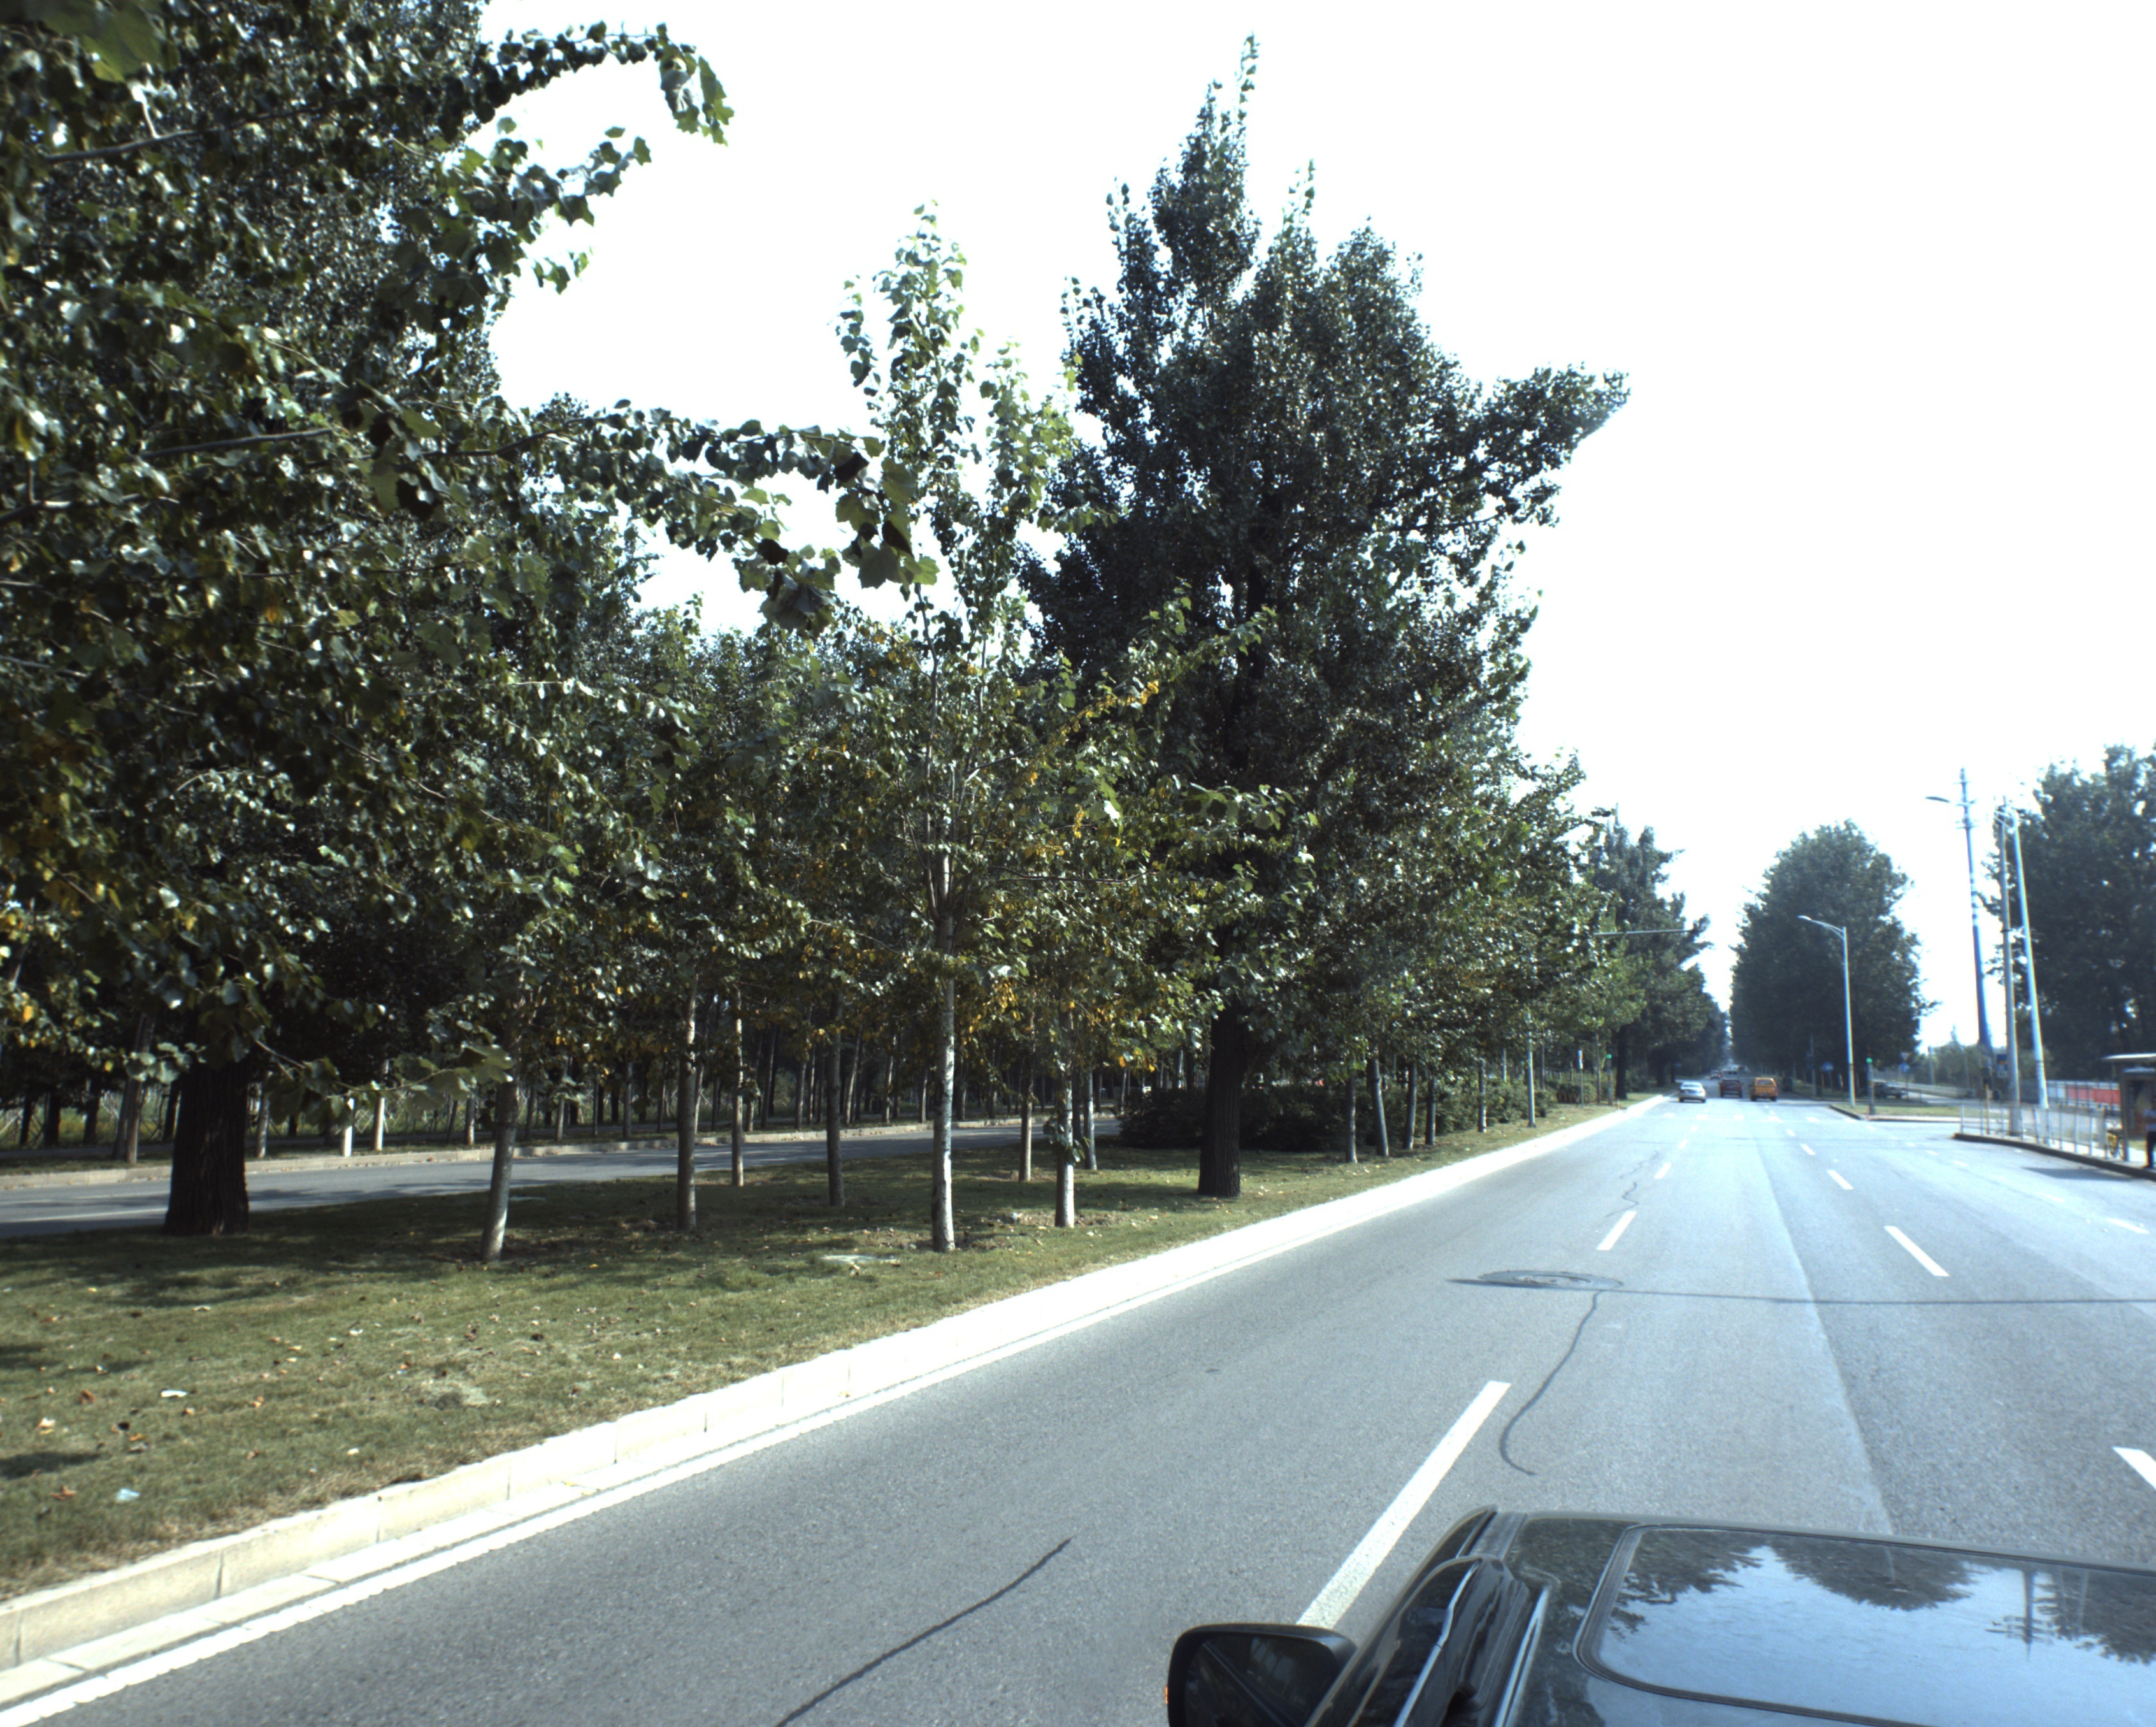
\includegraphics[width=\textwidth]{170908_061542022_Camera_5.jpg}
	\caption{Frame $n+1$}
\end{subfigure}
\begin{subfigure}{0.3\textwidth}
	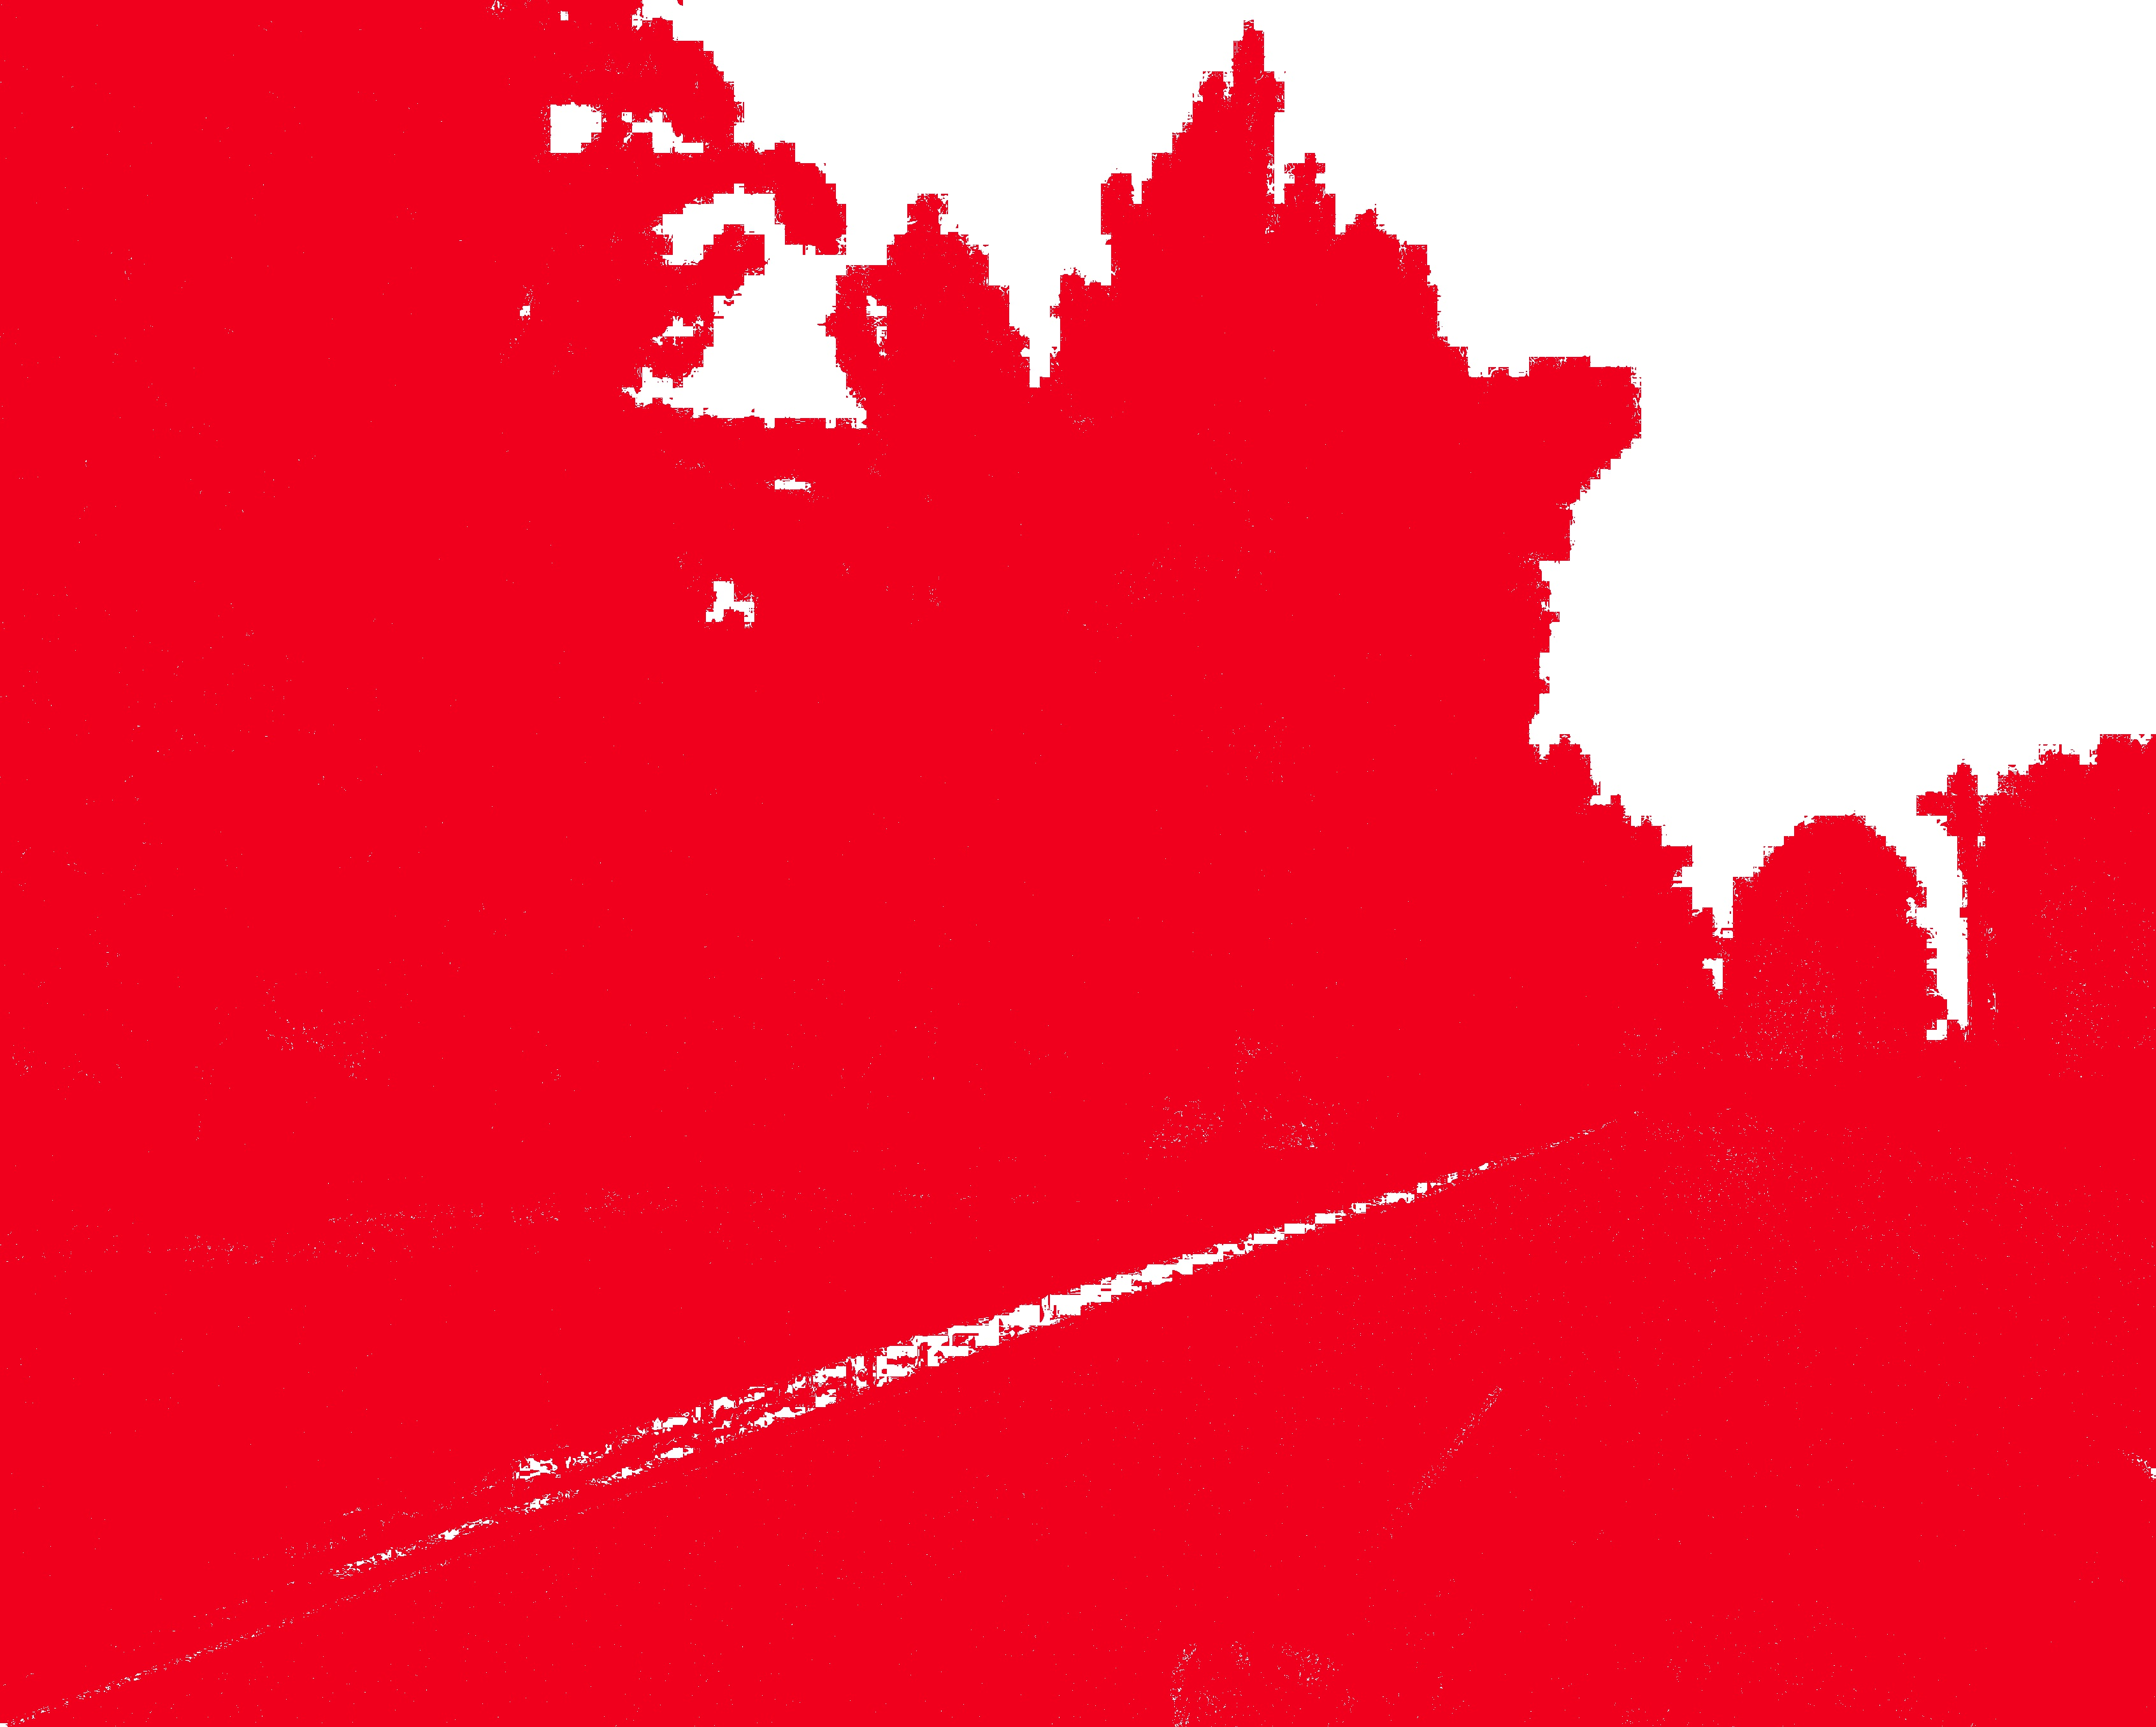
\includegraphics[width=\textwidth]{diff.jpg}
	\caption{Frame difference}
\end{subfigure}
\caption{Consecutive frames from a video stream and their difference at pixel
    level. The white region shows where the pixels have not changed.}
\label{fig:frames}
\end{figure}

\section{Sparse Direct Convolution}
\section{Evaluation}
\label{sec:eval}

\section{Conclusions}
\label{sec:conclusion}

\bibliographystyle{abbrv}
\nocite{*}
{\bibliography{report}}

\end{document}
